
\section{Internetes mérési eljárások}
%(5-6 oldal): Aktív/Passzív, Looking Glass, traceroute, ping, iperf
%whois szerverek
 
 
%hivatkozás a cikkre: http://www.ijcsit.com/docs/Volume%202/vol2issue4/ijcsit2011020402.pdf

Jelen fejezetben bemutatom a hálózati mérések motivációs hátterét, az egyes eljárások elméletét, végül az Internet tulajdonságait vizsgáló mérésekre térek ki.

Minden informatikai hálózat helyes működését mérésekkel szükséges ellenőrizni, így az Internetes hálózatét is. A hálózathoz fűződő viszonyaik alapján az egyes szereplők különböző motiváció alapján végeznek méréseket a hálózat viszonyainak felmérése érdekében. A \ref{tab:measurement-types} táblázatban\cite{networkMeasure} láthatóak az egyes motivációk és az azokhoz fűződő mérések. 

\input{measurement-table.txt}

Az egyes mérési eljárásokat a hálózat működésére való hatása alapján aktív és passzív kategóriába csoportosítjuk. Ezeken felül a legelterjedtebben a hibrid eljárásokat használják, amely magába foglal mindkét előző kategóriába tartozó méréseket is. A következő fejezetekben ezen eljárásokat mutatom be részletesebben.

\subsection{Aktív mérések}

Az aktív mérési eljárások alkalmazása visszahat a hálózatra, mivel új forgalmat hoz létre azon. Ez nem kívánt lehet, egyes esetekben azonban elkerülhetetlen, ha a végfelhasználó által észlelt hálózati viszonyokról szeretnénk megbizonyosodni.
%Ezen ellentétet leginkább a sávszélesség mérése mutatja be a legjobban. Az hálózat üzemeltetőjének egyik fontos szempontja megbizonyosodni hálózatának áteresztőképességéről, ahogy ez a \ref{tab:measurement-types} táblázatban is szerepel. Ennek érdekében azonban nem indít új 
Az aktív mérések két működési elv alapján működhetnek, vagy csak az adatfolyam forrása, vagy a nyelője is részt vesz a mérésben. Ez utóbbi esetben, a hálózatba küldött csomagok TTL\footnote{Time To Live - Élettartam} mezőjét használják fel, hogy az a cél cím elérése előtt az nullára csökkenjen, így \textit{Time To Live exceeded in transit} üzenet visszaküldésére kényszeríti a közbülső gépet, ahol nullázódott a TTL mező. Ezt az elvet használja a Traceroute mérőszoftver, amely egy cél cím felé vezető internetes útvonalat deríti fel ilyen üzenetekkel. Ennek a folyamatnak a sematikus működése látható a \ref{fig:traceroute-works} ábrán. Működéséhez szükséges az útvonalon lévő összes közbülső számítógépen engedélyezni a \textit{Time To Live exceeded in transit} küldését. Ennek hiányában nem működik a traceroute.
%ICMP TTL ping, iperf

\begin{figure}[h]
	\centering
	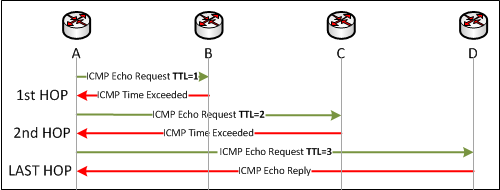
\includegraphics[width=0.7\textwidth, keepaspectratio]{figures/traceroute-works.png}
	\caption{A Traceroute útvonalfelderítés elve\protect\footnotemark}
	\label{fig:traceroute-works}
\end{figure}

\footnotetext{Forrás: \url{https://telconotes.wordpress.com/2013/02/08/how-traceroute-works/}}

Egy másik sokat használt mérőszoftver a ping, amely csak a célgéppel szemben tart fent elvárást, a közbülső gépekkel nem. Egy válaszkérő üzenetet küld, amelyre ha válasz érkezik akkor elérhetőnek számít a cél cím és a csomag körüljárási idejét is meg lehet állapítani.

Az eddig említett mérési elvek a hálózati eszközök szabványokban meghatározott működése alapján végeznek méréseket. A mérőrendszerben is alkalmazott iperf mérőszoftver viszont a cél címen telepített és futó példány segítségével képes csak a méréseket végrehajtani. Emiatt az üzemeltetése bonyolultabb, azonban információkban gazdag méréseket lehet végezni vele. Legfontosabb felhasználási funkciója a sávszélesség mérés.

\subsection{Passzív mérések}

Egyes esetekben szükségesek a vizsgálandó hálózatot nem terhelő vagy befolyásoló mérések. Ilyen esetekben passzív mérési eljárásokat alkalmaznak, melyek az áthaladó adatcsomagok vizsgálata alapján adnak visszajelzést a hálózat működéséről. Ilyen fajta méréseket főleg a hálózat üzemeltetői végeznek, mivel számukra egyszerű azokat végrehajtani a hálózati eszközök beállításával vagy az összekötő linkekre csatlakoztatott mérőeszközökkel. Egyik legelterjedtebb passzív hálózatmérési eljárás a Netflow, amelyet a Cisco fejlesztett ki, majd az IETF\footnote{Internet engineering task Force} is szabványosított. Működési alapelve, hogy a hálózati eszközökön az átmenő forgalmat egyes tulajdonságai alapján\footnote{Küldő/fogadó IP cím, küldő/fogadó port, használt protokoll, szolgáltatási osztály} folyamokba(flow) klasszifikálja, majd a generált forgalmuk historikus feljegyzésre kerül további elemzésre. 
%source/destination IP address, source/destination ports, protocol interface and class of service
% Netflow leírás: http://www.cisco.com/c/en/us/products/collateral/ios-nx-os-software/ios-netflow/prod_white_paper0900aecd80406232.html

\subsection{Hibrid mérések}

A korábban említett eljárások tulajdonságait ötvözik a hibrid hálózatmérési eljárások, melyek során mérési forgalmat generálnak a hálózatban, majd ezt passzív módon is megfigyelik. Ilyen módon egyszerre lehet információt kapni az egyes csomagok továbbítása során tapasztalt kezeléséről/életútjáról és a kapcsolat egészére vonatkozó tulajdonságokról. Ezzel a módszerrel lehet a legjobban megfigyelni a köztes elemek hatását a kapcsolat egészére.


\pagebreak

\subsection{További adatforrások}

Az Internet egészére vonatkozó mérések nehézségekkel néznek szembe annak mérete, folyamatos változása és tulajdonosi töredezettsége miatt. A következő \ref{internet-measurement} fejezetben ezen törekvéseket fogom bemutatni. Az alábbiakban ezek megértéséhez szolgáló további, az Internet tulajdonságait leíró adatforrásokat mutatok be.

Az előzőekben bemutatott IANA és a Regionális Internet Nyilvántartó szervezeteknek fontos feladata monitorozni az alájuk tartozó Internetes régiók működését. Az egyik legjobban bevált módszer a BGP protokoll hirdetéseinek a figyelése. Ezek a hirdetések az Autonóm Rendszerek közötti útvonalak helyen kiépítéséért felel. A BGP útvonalhirdetések megfigyelésére saját üzemeltetésű úgynevezett \mbox{Looking Glass\footnote{Angol jelentése tükör, lényegük hogy az Internet általuk látható felépítését közvetítik}} szervereket tartanak fent. 
Ezeknek a megfigyelési adatait pedig honlapjaikon\footnote{Példaként az RIPE honlapja: \url{https://atlas.ripe.net/landing/about/}} szabadon elérhetővé teszik, hogy további kutatók, üzemeltetők számára is átlátható legyen az Internet aktuális állapota.

Végső soron megemlítendőek még a WHOIS rendszerek, amelyek az egyes Internetes erőforrások tulajdonosairól adnak információkat, mint: IP címek, címtartományok, AS számok, DNS domének. Mindezen információforrások segítségével már komoly rálátással lehet bírni az Internetet alkotó Autonóm Rendszerekre.




%Looking Glass

%Cucc \cite{networkMeasure}.


